\section{Bottleneck-Features}\label{sec:bottleneck-features}

\begin{figure}
\centering
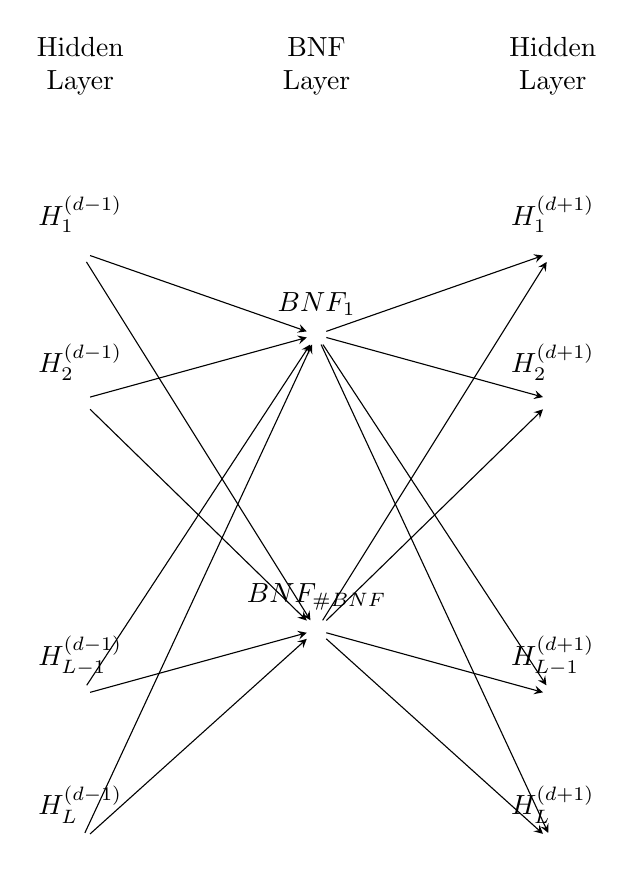
\begin{tikzpicture}[x=1.5cm, y=1.5cm, >=stealth]
% neurons
\foreach \m [count=\y] in {1,2,missing,3,4}
	\node [every neuron/.try, neuron \m/.try ] (hidden1-\m) at (0,2-\y*1.25) {};
\foreach \m [count=\y] in {1,missing,2}
	\node [every neuron/.try, neuron \m/.try ] (BNF-\m) at (2,1.3-\y*1.25) {};
\foreach \m [count=\y] in {1,2,missing,3,4}
	\node [every neuron/.try, neuron \m/.try ] (hidden2-\m) at (4,2-\y*1.25) {};

% neuron labels
\foreach \l [count=\i] in {1,2,L-1,...,L-1,L}
	\node [above] at (hidden1-\i.north) {$H^{(d-1)}_{\l}$};
\foreach \l [count=\i] in {1,\#BNF}
	\node [above] at (BNF-\i.north) {$BNF_{\l}$};
\foreach \l [count=\i] in {1,2,L-1,...,L-1,L}
	\node [above] at (hidden2-\i.north) {$H^{(d+1)}_{\l}$};

% neuron connection
\foreach \i in {1,...,4}
	\foreach \j in {1,...,2}
		\draw [->] (hidden1-\i) -- (BNF-\j);
\foreach \i in {1,...,2}
			\foreach \j in {1,...,4}
				\draw [->] (BNF-\i) -- (hidden2-\j);

% layer labels
\foreach \l [count=\x from 0] in {Hidden, BNF, Hidden}
	\node [align=center, above] at (\x*2,2) {\l \\ Layer};

\end{tikzpicture}
\caption{Neural network with Bottleneck features}
\label{fig:bottleneck-features}
\end{figure}
